%% bare_conf.tex
%% V1.3
%% 2007/01/11
%% by Michael Shell
%% See:
%% http://www.michaelshell.org/
%% for current contact information.
%%
%% This is a skeleton file demonstrating the use of IEEEtran.cls
%% (requires IEEEtran.cls version 1.7 or later) with an IEEE conference paper.
%%
%% Support sites:
%% http://www.michaelshell.org/tex/ieeetran/
%% http://www.ctan.org/tex-archive/macros/latex/contrib/IEEEtran/
%% and
%% http://www.ieee.org/

%%*************************************************************************
%% Legal Notice:
%% This code is offered as-is without any warranty either expressed or
%% implied; without even the implied warranty of MERCHANTABILITY or
%% FITNESS FOR A PARTICULAR PURPOSE! 
%% User assumes all risk.
%% In no event shall IEEE or any contributor to this code be liable for
%% any damages or losses, including, but not limited to, incidental,
%% consequential, or any other damages, resulting from the use or misuse
%% of any information contained here.
%%
%% All comments are the opinions of their respective authors and are not
%% necessarily endorsed by the IEEE.
%%
%% This work is distributed under the LaTeX Project Public License (LPPL)
%% ( http://www.latex-project.org/ ) version 1.3, and may be freely used,
%% distributed and modified. A copy of the LPPL, version 1.3, is included
%% in the base LaTeX documentation of all distributions of LaTeX released
%% 2003/12/01 or later.
%% Retain all contribution notices and credits.
%% ** Modified files should be clearly indicated as such, including  **
%% ** renaming them and changing author support contact information. **
%%
%% File list of work: IEEEtran.cls, IEEEtran_HOWTO.pdf, bare_adv.tex,
%%                    bare_conf.tex, bare_jrnl.tex, bare_jrnl_compsoc.tex
%%*************************************************************************

% *** Authors should verify (and, if needed, correct) their LaTeX system  ***
% *** with the testflow diagnostic prior to trusting their LaTeX platform ***
% *** with production work. IEEE's font choices can trigger bugs that do  ***
% *** not appear when using other class files.                            ***
% The testflow support page is at:
% http://www.michaelshell.org/tex/testflow/



% Note that the a4paper option is mainly intended so that authors in
% countries using A4 can easily print to A4 and see how their papers will
% look in print - the typesetting of the document will not typically be
% affected with changes in paper size (but the bottom and side margins will).
% Use the testflow package mentioned above to verify correct handling of
% both paper sizes by the user's LaTeX system.
%
% Also note that the "draftcls" or "draftclsnofoot", not "draft", option
% should be used if it is desired that the figures are to be displayed in
% draft mode.
%
\documentclass[10pt, conference, compsocconf]{IEEEtran}
% Add the compsocconf option for Computer Society conferences.
%
% If IEEEtran.cls has not been installed into the LaTeX system files,
% manually specify the path to it like:
% \documentclass[conference]{../sty/IEEEtran}





% Some very useful LaTeX packages include:
% (uncomment the ones you want to load)


% *** MISC UTILITY PACKAGES ***
%
%\usepackage{ifpdf}
% Heiko Oberdiek's ifpdf.sty is very useful if you need conditional
% compilation based on whether the output is pdf or dvi.
% usage:
% \ifpdf
%   % pdf code
% \else
%   % dvi code
% \fi
% The latest version of ifpdf.sty can be obtained from:
% http://www.ctan.org/tex-archive/macros/latex/contrib/oberdiek/
% Also, note that IEEEtran.cls V1.7 and later provides a builtin
% \ifCLASSINFOpdf conditional that works the same way.
% When switching from latex to pdflatex and vice-versa, the compiler may
% have to be run twice to clear warning/error messages.






% *** CITATION PACKAGES ***
%
%\usepackage{cite}
% cite.sty was written by Donald Arseneau
% V1.6 and later of IEEEtran pre-defines the format of the cite.sty package
% \cite{} output to follow that of IEEE. Loading the cite package will
% result in citation numbers being automatically sorted and properly
% "compressed/ranged". e.g., [1], [9], [2], [7], [5], [6] without using
% cite.sty will become [1], [2], [5]--[7], [9] using cite.sty. cite.sty's
% \cite will automatically add leading space, if needed. Use cite.sty's
% noadjust option (cite.sty V3.8 and later) if you want to turn this off.
% cite.sty is already installed on most LaTeX systems. Be sure and use
% version 4.0 (2003-05-27) and later if using hyperref.sty. cite.sty does
% not currently provide for hyperlinked citations.
% The latest version can be obtained at:
% http://www.ctan.org/tex-archive/macros/latex/contrib/cite/
% The documentation is contained in the cite.sty file itself.






% *** GRAPHICS RELATED PACKAGES ***
%
\ifCLASSINFOpdf
  \usepackage[pdftex]{graphicx}
  % declare the path(s) where your graphic files are
  % \graphicspath{{../pdf/}{../jpeg/}}
  % and their extensions so you won't have to specify these with
  % every instance of \includegraphics
  \DeclareGraphicsExtensions{.pdf,.jpeg,.png}
\else
  % or other class option (dvipsone, dvipdf, if not using dvips). graphicx
  % will default to the driver specified in the system graphics.cfg if no
  % driver is specified.
  % \usepackage[dvips]{graphicx}
  % declare the path(s) where your graphic files are
  % \graphicspath{{../eps/}}
  % and their extensions so you won't have to specify these with
  % every instance of \includegraphics
  % \DeclareGraphicsExtensions{.eps}
\fi
% graphicx was written by David Carlisle and Sebastian Rahtz. It is
% required if you want graphics, photos, etc. graphicx.sty is already
% installed on most LaTeX systems. The latest version and documentation can
% be obtained at: 
% http://www.ctan.org/tex-archive/macros/latex/required/graphics/
% Another good source of documentation is "Using Imported Graphics in
% LaTeX2e" by Keith Reckdahl which can be found as epslatex.ps or
% epslatex.pdf at: http://www.ctan.org/tex-archive/info/
%
% latex, and pdflatex in dvi mode, support graphics in encapsulated
% postscript (.eps) format. pdflatex in pdf mode supports graphics
% in .pdf, .jpeg, .png and .mps (metapost) formats. Users should ensure
% that all non-photo figures use a vector format (.eps, .pdf, .mps) and
% not a bitmapped formats (.jpeg, .png). IEEE frowns on bitmapped formats
% which can result in "jaggedy"/blurry rendering of lines and letters as
% well as large increases in file sizes.
%
% You can find documentation about the pdfTeX application at:
% http://www.tug.org/applications/pdftex





% *** MATH PACKAGES ***
%
\usepackage[cmex10]{amsmath}
% A popular package from the American Mathematical Society that provides
% many useful and powerful commands for dealing with mathematics. If using
% it, be sure to load this package with the cmex10 option to ensure that
% only type 1 fonts will utilized at all point sizes. Without this option,
% it is possible that some math symbols, particularly those within
% footnotes, will be rendered in bitmap form which will result in a
% document that can not be IEEE Xplore compliant!
%
% Also, note that the amsmath package sets \interdisplaylinepenalty to 10000
% thus preventing page breaks from occurring within multiline equations. Use:
%\interdisplaylinepenalty=2500
% after loading amsmath to restore such page breaks as IEEEtran.cls normally
% does. amsmath.sty is already installed on most LaTeX systems. The latest
% version and documentation can be obtained at:
% http://www.ctan.org/tex-archive/macros/latex/required/amslatex/math/





% *** SPECIALIZED LIST PACKAGES ***
%
%\usepackage{algorithmic}
% algorithmic.sty was written by Peter Williams and Rogerio Brito.
% This package provides an algorithmic environment fo describing algorithms.
% You can use the algorithmic environment in-text or within a figure
% environment to provide for a floating algorithm. Do NOT use the algorithm
% floating environment provided by algorithm.sty (by the same authors) or
% algorithm2e.sty (by Christophe Fiorio) as IEEE does not use dedicated
% algorithm float types and packages that provide these will not provide
% correct IEEE style captions. The latest version and documentation of
% algorithmic.sty can be obtained at:
% http://www.ctan.org/tex-archive/macros/latex/contrib/algorithms/
% There is also a support site at:
% http://algorithms.berlios.de/index.html
% Also of interest may be the (relatively newer and more customizable)
% algorithmicx.sty package by Szasz Janos:
% http://www.ctan.org/tex-archive/macros/latex/contrib/algorithmicx/




% *** ALIGNMENT PACKAGES ***
%
%\usepackage{array}
% Frank Mittelbach's and David Carlisle's array.sty patches and improves
% the standard LaTeX2e array and tabular environments to provide better
% appearance and additional user controls. As the default LaTeX2e table
% generation code is lacking to the point of almost being broken with
% respect to the quality of the end results, all users are strongly
% advised to use an enhanced (at the very least that provided by array.sty)
% set of table tools. array.sty is already installed on most systems. The
% latest version and documentation can be obtained at:
% http://www.ctan.org/tex-archive/macros/latex/required/tools/


%\usepackage{mdwmath}
%\usepackage{mdwtab}
% Also highly recommended is Mark Wooding's extremely powerful MDW tools,
% especially mdwmath.sty and mdwtab.sty which are used to format equations
% and tables, respectively. The MDWtools set is already installed on most
% LaTeX systems. The lastest version and documentation is available at:
% http://www.ctan.org/tex-archive/macros/latex/contrib/mdwtools/


% IEEEtran contains the IEEEeqnarray family of commands that can be used to
% generate multiline equations as well as matrices, tables, etc., of high
% quality.


%\usepackage{eqparbox}
% Also of notable interest is Scott Pakin's eqparbox package for creating
% (automatically sized) equal width boxesreaka "natural width parboxes".
% Available at:
% http://www.ctan.org/tex-archive/macros/latex/contrib/eqparbox/





% *** SUBFIGURE PACKAGES ***
%\usepackage[tight,footnotesize]{subfigure}
% subfigure.sty was written by Steven Douglas Cochran. This package makes it
% easy to put subfigures in your figures. e.g., "Figure 1a and 1b". For IEEE
% work, it is a good idea to load it with the tight package option to reduce
% the amount of white space around the subfigures. subfigure.sty is already
% installed on most LaTeX systems. The latest version and documentation can
% be obtained at:
% http://www.ctan.org/tex-archive/obsolete/macros/latex/contrib/subfigure/
% subfigure.sty has been superceeded by subfig.sty.



%\usepackage[caption=false]{caption}
%\usepackage[font=footnotesize]{subfig}
% subfig.sty, also written by Steven Douglas Cochran, is the modern
% replacement for subfigure.sty. However, subfig.sty requires and
% automatically loads Axel Sommerfeldt's caption.sty which will override
% IEEEtran.cls handling of captions and this will result in nonIEEE style
% figure/table captions. To prevent this problem, be sure and preload
% caption.sty with its "caption=false" package option. This is will preserve
% IEEEtran.cls handing of captions. Version 1.3 (2005/06/28) and later 
% (recommended due to many improvements over 1.2) of subfig.sty supports
% the caption=false option directly:
%\usepackage[caption=false,font=footnotesize]{subfig}
%
% The latest version and documentation can be obtained at:
% http://www.ctan.org/tex-archive/macros/latex/contrib/subfig/
% The latest version and documentation of caption.sty can be obtained at:
% http://www.ctan.org/tex-archive/macros/latex/contrib/caption/




% *** FLOAT PACKAGES ***
%
%\usepackage{fixltx2e}
% fixltx2e, the successor to the earlier fix2col.sty, was written by
% Frank Mittelbach and David Carlisle. This package corrects a few problems
% in the LaTeX2e kernel, the most notable of which is that in current
% LaTeX2e releases, the ordering of single and double column floats is not
% guaranteed to be preserved. Thus, an unpatched LaTeX2e can allow a
% single column figure to be placed prior to an earlier double column
% figure. The latest version and documentation can be found at:
% http://www.ctan.org/tex-archive/macros/latex/base/



%\usepackage{stfloats}
% stfloats.sty was written by Sigitas Tolusis. This package gives LaTeX2e
% the ability to do double column floats at the bottom of the page as well
% as the top. (e.g., "\begin{figure*}[!b]" is not normally possible in
% LaTeX2e). It also provides a command:
%\fnbelowfloat
% to enable the placement of footnotes below bottom floats (the standard
% LaTeX2e kernel puts them above bottom floats). This is an invasive package
% which rewrites many portions of the LaTeX2e float routines. It may not work
% with other packages that modify the LaTeX2e float routines. The latest
% version and documentation can be obtained at:
% http://www.ctan.org/tex-archive/macros/latex/contrib/sttools/
% Documentation is contained in the stfloats.sty comments as well as in the
% presfull.pdf file. Do not use the stfloats baselinefloat ability as IEEE
% does not allow \baselineskip to stretch. Authors submitting work to the
% IEEE should note that IEEE rarely uses double column equations and
% that authors should try to avoid such use. Do not be tempted to use the
% cuted.sty or midfloat.sty packages (also by Sigitas Tolusis) as IEEE does
% not format its papers in such ways.





% *** PDF, URL AND HYPERLINK PACKAGES ***
%
%\usepackage{url}
% url.sty was written by Donald Arseneau. It provides better support for
% handling and breaking URLs. url.sty is already installed on most LaTeX
% systems. The latest version can be obtained at:
% http://www.ctan.org/tex-archive/macros/latex/contrib/misc/
% Read the url.sty source comments for usage information. Basically,
% \url{my_url_here}.





% *** Do not adjust lengths that control margins, column widths, etc. ***
% *** Do not use packages that alter fonts (such as pslatex).         ***
% There should be no need to do such things with IEEEtran.cls V1.6 and later.
% (Unless specifically asked to do so by the journal or conference you plan
% to submit to, of course. )


% correct bad hyphenation here
\hyphenation{op-tical net-works semi-conduc-tor}

% booktabs (is this allowed?)
\usepackage{booktabs}

% some text vars
\usepackage{xspace}
\newcommand{\TI}{ASILD1\xspace}
\newcommand{\ST}{ASILD2\xspace}
\newcommand{\NXP}{QM1\xspace}

\newcommand{\unroll}{\texttt{unroll}\xspace}
\newcommand{\auth}{\texttt{auth}\xspace}
\newcommand{\jtag}{JTAG\xspace}

% code (this is allowed, right?)
\usepackage{listings}
\lstset{
basicstyle=\ttfamily
}

% for vertically centered ~ (texttildelow)
\usepackage{textcomp}

\begin{document}
%
% paper title
% can use linebreaks \\ within to get better formatting as desired
\title{Safety != Security \\ {\large On the resilience of ASIL-D certified microcontrollers against fault injection attacks}}


% author names and affiliations
% use a multiple column layout for up to two different
% affiliations

%\author{\IEEEauthorblockN{Nils Wiersma, Ramiro Pareja}
%\IEEEauthorblockA{Security Lab\\
%Riscure\\
%Delft, the Netherlands\\
%Email: \{wiersma, pareja\} @ riscure.com}

%}

% conference papers do not typically use \thanks and this command
% is locked out in conference mode. If really needed, such as for
% the acknowledgment of grants, issue a \IEEEoverridecommandlockouts
% after \documentclass

% for over three affiliations, or if they all won't fit within the width
% of the page, use this alternative format:
% 
%\author{\IEEEauthorblockN{Michael Shell\IEEEauthorrefmark{1},
%Homer Simpson\IEEEauthorrefmark{2},
%James Kirk\IEEEauthorrefmark{3}, 
%Montgomery Scott\IEEEauthorrefmark{3} and
%Eldon Tyrell\IEEEauthorrefmark{4}}
%\IEEEauthorblockA{\IEEEauthorrefmark{1}School of Electrical and Computer Engineering\\
%Georgia Institute of Technology,
%Atlanta, Georgia 30332--0250\\ Email: see http://www.michaelshell.org/contact.html}
%\IEEEauthorblockA{\IEEEauthorrefmark{2}Twentieth Century Fox, Springfield, USA\\
%Email: homer@thesimpsons.com}
%\IEEEauthorblockA{\IEEEauthorrefmark{3}Starfleet Academy, San Francisco, California 96678-2391\\
%Telephone: (800) 555--1212, Fax: (888) 555--1212}
%\IEEEauthorblockA{\IEEEauthorrefmark{4}Tyrell Inc., 123 Replicant Street, Los Angeles, California 90210--4321}}




% use for special paper notices
%\IEEEspecialpapernotice{(Invited Paper)}




% make the title area
\maketitle


\begin{abstract}
With the ever increasing amount of electronic components in vehicles and in particular the amount of complex autonomous actions that these components perform, security topics become more and more important in the automotive industry. 
Not only from a business point of view, as valuable IP assets are contained within these components, but also from a safety point of view, especially when vulnerabilities lead to remotely exploitable attacks.
Logical attacks in this field are abundant, but attacks using hardware centered techniques such as fault injection are underrepresented. Researchers and professionals often pay no attention in these attacks because they require physical access to the chip, ignoring that the assets obtained (e.g. firmware, keys, etc.) can be used later to prepare a remote attack.      

This work aims to address the lack of attention on fault injection attacks by investigating two modern microcontroller units that receive the highest safety assurance rating (ASIL-D) of the ISO 26262 automotive standard. This is done in both a theoretical characterization setup and a more realistic setup where debugging interfaces are targeted.
The results obtained from these setups show that the mechanisms implemented to adhere to this maximum safety rating do not adequately protect against fault injection attacks and are therefore insufficient to ensure security by themselves -- additional countermeasures are required. Each setup required approximately one week of preparation, but once the attacker finds the optimal fault injection parameters, the attack can be repeated in less than an hour. We provide some recommendations on what type of countermeasures should be considered to improve the security with respect to fault injection attacks and also provide several pointers to continue the security research in this area.

\end{abstract}

\begin{IEEEkeywords}
fault injection; power analysis; ASIL; ISO-26262; safety mechanisms; countermeasures; lockstep; JTAG

\end{IEEEkeywords}


% For peer review papers, you can put extra information on the cover
% page as needed:
% \ifCLASSOPTIONpeerreview
% \begin{center} \bfseries EDICS Category: 3-BBND \end{center}
% \fi
%
% For peerreview papers, this IEEEtran command inserts a page break and
% creates the second title. It will be ignored for other modes.
\IEEEpeerreviewmaketitle



\section{Introduction}
% no \IEEEPARstart
Microcontroller units (MCU) form the foundation of the modern car. They are used to implement functionalities that can be as simple as opening the window when a button is pressed, or as complicated as Vehicle to Vehicle communications and autonomous driving systems. They can perform non-critical tasks such as controlling the windscreen wipers or extremely critical ones like making sure airbags are deployed in case of an emergency. 
 
Over the last two decades the number of electronic controllers in vehicles has increased, making evident the need of ensuring the reliability and safety of these MCUs. 
The ISO 26262 standard \cite{iso26262} -- in particular part 10, Annex. A and part 5, Annex. D -- recognizes the pivotal part that MCUs play in the ecosystem of a vehicle and establishes a framework for the development of safe automotive electronic systems. Part 5 of the standard gives a number of examples of safety mechanisms that can be implemented to mitigate different electric faults that could affect the operation of an electronic system and consequently threaten the safety of the vehicle's passengers. Although these examples and recommendations intend to protect against faults occurring during normal use of the vehicle, some of these safety measures are also often recommended in the security literature as countermeasures against fault injection (FI) attacks (e.g. \cite{bar-el_sorcerers_2006-1}).  Previous work \cite{tummeltshammer_power_2009} shows that voltage glitching can be prevented by these kinds of mechanisms.
It is therefore easily taken for granted that MCUs implementing ISO 26262 recommendations (i.e. ASIL-D chips) are also protected against FI attacks.

This paper summarizes our investigations into 
the effectiveness of the ISO 26262's recommendations as a means to resist against FI attacks. We first determine the resistance to FI of two ASIL-D certified MCUs and a standard (non-ASIL) automotive MCU in a controlled test environment. Next, we explore the risks of FI on ASIL-D chips by attacking the debug interface protection mechanism in our targets. Finally, we discuss the consequences and threats these attacks pose in the automotive context and provide recommendations for mitigating the aforementioned threats.


\section{Automotive context, ISO 26262 and fault injection}
Automotive standards and literature, especially with regards to hardware, primarily deal with safety. In this context, faults are considered as an unintended, abnormal and often random condition caused by the hostile environment in which the hardware resides (e.g. high temperatures, noisy power supply, vibrations, electromagnetic (EM) pulses produced by coils, etc.). ISO 26262 provides recommendations to mitigate and minimize the impact of these unintentional faults and defines the Automotive Safety Integrity Level (ASIL) risk classification scheme from level A through D (see Table \ref{tab:ASIL}). ASIL-D complying MCUs are required to adhere to the most stringent requirements on safety and fault-tolerance in order to achieve absence of unreasonable risk. A fifth level, QM, is defined for parts that only require basic quality management. FI is mentioned in the ISO 26262 only as a method of testing the compliance of the ASIL requirements.  

\begin{table}[!t]
    \caption{ASIL categories} 
    \label{tab:ASIL}
    \centering
    \begin{tabular}{rlcccr}
    \toprule
    Category        & QM  & ASIL-A & ASIL-B & ASIL-C & ASIL-D \\
                    & &&&&\\
    Assurance level &   \multicolumn{5}{c}{Low \ \   $\xrightarrow{\hspace*{4cm}}$ \ \ High} \\
    \bottomrule
    \end{tabular}
\end{table}

When shifting to the domain of security, faults are no longer the effect of random and unintended events. They are the result of \emph{glitches} in the environment that are deliberately placed, precisely timed and carefully tuned by an attacker with the purpose causing unintended behavior -- the \emph{fault} -- which is leveraged to compromise the chip security. These FI attacks are in general used to alter the program flow or the processed data. If this is possible, an attacker could, for example, bypass the Secure Boot process by skipping the signature verification and executing unauthenticated code \cite{timmers_controlling_2016}, bypass the authentication of the UDS protocol to extract the firmware or recover cryptographic keys using a Differential Fault Analysis (DFA) attack \cite{biehl_differential_2000,boneh_importance_2001,giraud_dfa_2004}. 

For this work, two techniques of injecting faults have been considered: voltage glitching -- a fast variation of the power supply voltage -- and transient EM glitching -- a strong and localized EM pulse. A voltage glitching device is cheap (tools can be bought for even less than 200€) but the attack is not localized, as it affects the entire chip, and requires modifying the target board by removing the capacitors. EM glitching on the other hand requires no modifications on the board and the glitches are local (i.e. they affect a small area of the chip) but the equipment required is more expensive. 


\section{Targets}
To investigate the effectiveness of safety mechanisms as countermeasures against FI attacks, two ASIL-D certified MCUs that implement these mechanisms have been selected, from two different
manufacturers. 
Although we believe that we would have obtained similar results with any other ASIL-D MCU in the market, we omit the chip models because we are still in the process of disclosing the findings to the manufacturers in a coordinated manner.

The first target, codenamed \TI, implements an ARM Cortex-R4 core and the second target, codenamed \ST, a PowerPC e200. These two targets were selected because they represent two of the most prevalent architectures in the safety electronic industry. For reference and comparison, a non-ASIL target has been chosen, code-named \NXP. This target implements an ARM Cortex-M0 and can be used for simple applications which require only the basic QM rating.

Of all the safety mechanisms implemented in ASIL-D MCUs, we are only interested in investigating the ones that have an effect on transient faults as they could also mitigate the glitches used by an FI attacker. In both selected targets these mechanisms include a dual core CPU in lockstep configuration (or `Simple Time Redundancy with Comparison') and memories with error correction codes (ECC) and parity bits, as recommended by ISO 26262 part 5. 

\subsection{FI tools}
Commercially available hardware 
and software 
is used for injecting glitches.
The central piece to the hardware setup is the VCGlitcher, an FPGA powered device capable of generating two types of glitches: voltage glitches with 2ns of precision; or input to an EM pulse emitter device for the purpose of EM glitching. During the characterization experiments where the target is fully under our control and running our firmware, a GPIO pin of the target is used to generate a signal that triggers the VCGlitcher. In the experiments where the target is not controlled, the icWaves tool is used. This device analyzes the power consumption of the target and generates a trigger signal when a programmable reference pattern is detected. The setup is controlled by a Windows host machine running the Inspector FI software.

\subsection{Target preparations}
Standard low-cost development boards are used as target for the three MCUs under test. For voltage glitching, the power traces of the printed circuit board (PCB) are modified where needed. The purpose of this modification is to isolate the MCU power supply from the rest of the circuit, so the voltage glitch affects only the MCU and not the other components on the PCB. Additionally, the decoupling capacitors of the MCU are removed as they affect the shape of the voltage glitch. For EM glitching, no modifications to the boards are needed.

In order to determine the effect of the glitch, in particular whether or not it caused a useful fault, targets are programmed with software that outputs the contents of several internal registers over UART. This allows us to determine whether or not a particular safety mechanism has been triggered. 

\subsection{Glitch parameters}
The effectiveness of a glitch depends on the moment in time when the glitch is injected and the shape of the glitch. These can be modeled through parameters like the glitch length, glitch intensity (voltage or EM field) and time offset from the trigger signal. In the case of EM glitching, the point on the chip surface where the EM field is applied is also important.

A glitch can have various effects on a target, depending on the aforementioned parameters. A glitch is considered successful when it causes a fault in the target that results in the behavior that the attacker is looking for (e.g. bypassing a check). A glitch can also result in crashes or unexpected behavior. In this work, special attention is paid to glitches that are detected (or not) by the safety mechanisms under investigation. When a glitch is mentioned as detected, it means that it was detected by one or more of these mechanisms. Classification is based on internal error registers and externally observable error output pins.

The methodology used for finding the optimal parameters -- that is, those with the highest success rate -- involves running multiple FI campaigns. In each campaign, thousands of glitches are attempted while varying the parameters within a certain range. The initial FI campaign runs on very broad parameters. The parameters of the successful glitches found are used to restrict the search range in the next campaign and after few iterations of this process the optimal parameters are found.


\section{Characterization}
\label{sec:char}
The general effectiveness of the safety mechanisms in preventing FI is investigated in a characterization test. This test involves two experiments in a controlled environment: a very simple setup featuring a set of unrolled addition instructions and a more intricate scenario that employs a conditional branch.

\subsection{Scenario 1 -- \unroll}
In the first experiment, \unroll, a sequence of increment instructions is performed on the same CPU register. This should produce a predictable final value in the counter register. The final value of the register is sent over a serial connection at the end of the sequence together with the internal state of the MCU and its fault detectors. A pseudo code version of this setup is given in Listing 1. 
\begin{lstlisting}[caption={\unroll scenario pseudo code}, captionpos=b]
trigger_up()
asm(add r1 #1)
asm(add r1 #1)
...
asm(add r1 #1)
asm(add r1 #1)
trigger_down()
send_serial(r1)
\end{lstlisting}
A successful glitch affects the value of \texttt{r1} by altering the content of the register itself or by changing the code flow and skipping one (or more) increment instruction(s), without triggering the fault detectors.

\subsection{Scenario 2 -- \auth}
\unroll is one of the most basic experiments that can be performed and a good starting point for characterizing MCUs. The goal of the test is to confirm that the target is sensitive to FI. If successful glitches are found, additional experimentation should be done involving more realistic scenarios. The additional experiment chosen in this work is a conditional branch setup -- \auth. In this experiment an \texttt{if}-statement determines the program flow, simulating a situation where an authentication check is performed, as shown in Listing 2.
\begin{lstlisting}[caption={\auth scenario pseudo code}, captionpos=b]
flag = 1
...
trigger_up()
if (flag == 0):
    send_serial_authenticated()
else
    send_serial_denied()
trigger_down()
\end{lstlisting}
A successful glitch affects the \texttt{if}-statement so the unintended branch -- \texttt{send\_serial\_authenticated()} -- is executed.

\subsection{Results}
\begin{table}[!t]
\caption{The success rates of the characterization experiments} 
\label{tab:char-experiments}
\centering
\begin{tabular}{l cc cc}
\toprule
         & \multicolumn{2}{c}{\unroll}  
         & \multicolumn{2}{c}{\auth}       \\
           
           \cmidrule(lr){2-3}  \cmidrule(lr){4-5}        
         
         & \multicolumn{1}{c}{Power}                        & \multicolumn{1}{c}{EM}  
         & \multicolumn{1}{c}{Power}                        & \multicolumn{1}{c}{EM}                              
               \\
        \cmidrule(lr){1-5}
\TI      & 87\%   
         & 0.2\%      
         & 60\%   
         & 0.2\%      
         \\
\ST 
         & 0\%                  
         & 18\%                
         & N/A      
         & 57\%                 
         \\
\NXP 
         & 100\%                  
         & N/A               
         & N/A      
         & N/A                 
         \\
\bottomrule
\end{tabular}
\end{table}
These two experiments were prepared and performed on the three different targets over a period of three weeks. A total of \texttildelow720,000, \texttildelow550,000 and \texttildelow900,000 glitches were injected in the \TI, \ST and \NXP respectively. The final results of the characterization part of this work are given in Table \ref{tab:char-experiments}. These percentages represent the rates of successful and undetected glitches obtained for the last FI campaign of each characterization experiment, after finding and using the most effective glitch parameters. Around 10,000 glitches were injected in each of these last FI campaigns. Other campaigns -- not reflected in this table -- were able to successfully affect   the program execution but were detected by the MCU safety mechanisms.   

For \TI, EM glitching was attempted only to verify its feasibility. The EM FI campaigns did not attempt to find the most EM sensitive point in the chip surface and the optimal parameters. Therefore only a 0.2\% of success rate was achieved after one day of testing. If the optimal parameters are found and used, it is reasonable to expect a success rate similar to voltage glitching.

On \ST, voltage glitching proved to be ineffective in the \unroll experiment. Furthermore, none of our glitches were reported as detected. We find a possible explanation in the internal power distribution and the on-chip voltage regulator that could be filtering the glitches. We did not try voltage glitching in the following \ST experiments, limiting them to EM glitching. 
\NXP is also characterized, by using the unroll experiment and voltage glitching. Due to a high  initial success rate, no more characterization experiments are run as similar results are expected in the rest of the tests.

Analyzing the information collected during the \TI campaigns, we find that the most effective detection mechanism is the lockstep output comparison, which was triggered in 84\% to 98\% of the detected glitches, varying from experiment to experiment. Flash and RAM parity errors were triggered in 18\% to 25\% of the detected glitches. Other safety mechanisms were triggered in less than 3.5\% of the detected glitches. Note that a glitch can trigger many detection mechanisms at the same time. The \ST target does not report faults with enough detail to analyze the effectiveness of the different safety mechanisms.

Contrary to our initial expectations, all the previous described experiments succeeded while using a single glitch. Moreover, when using two glitches separated by the same number of clock cycles as the lockstep delay, the success rate decreases drastically.

The primary conclusion to be drawn from these characterization experiments is that it is possible to find glitch parameters for both \TI and \ST which result in a relatively high rate of successful glitches, without triggering any detection mechanism. 
Lacking a detailed insight into these mechanisms, it is hard to determine  with certainty the cause of them failing to detect more glitch attempts. 
We suspect that the cause could be in the fact that both ASIL-D targets implement lockstep configurations that only compare the CPU output signals and not the internal CPU state. Both targets use a two-clock cycles delay lockstep with pipelined CPUs. This suggests that an injected glitch could affect the same instruction being executed in the two lockstep cores but in different stages of the pipeline, resulting in similar output signals and not triggering the lockstep error. Furthermore, the fact that only output signals are taken into account means that if faults are injected in memory shared between the cores -- a part of the system that is not run in lockstep -- both cores will execute the same faulty instructions or operate on the same faulty values. Error control schemes for these memories should offer a solution here, but they might be insufficient according these results.


\section{Breaking JTAG protection}
\label{sec:jtag}
Previously discussed characterization experiments show that it is possible to use FI on ASIL-D MCUs to affect the code execution flow and bypass instructions, even if lockstep processing units and ECC protected memories are used. These experiments are run in a white-box manner in a controlled environment with full control over the software, including a trigger signal. Real attacks are typically executed in a black-box manner where the attacker has no control over the CPU and no access to the code.  In order to have a better understanding of the risks that FI attacks pose on a real application, a new FI experiment that represents a non-controlled environment is prepared. As debug interface access is one of the first assets that an attacker tries to obtain, the resistance of the debug interface protection mechanisms present in our targets is assessed against FI attacks in this new experiment.

Most modern MCUs have a permanent protection mechanism for closing the debug interfaces. This protection is usually enabled at the end of the manufacturing process of the embedded system in order to protect the firmware contained in the MCU. It is a common practice for many semiconductor manufacturers to implement this debug interface protection in the ROM code executed at boot time, before the application firmware is executed. This ROM usually reads the protection configuration from an one-time programmable (OTP) memory section or a word in the internal flash and configures the registers of the debug interface module accordingly. An attacker using FI to bypass the configuration read or to disturb the debug module configuration moment would effectively unlock the debug interface on a protected device, which is considered here as successful. 

Successful FI attacks rely on reliable trigger signals to ensure precise timing of a glitch. In the characterization experiments, the trigger signal was generated by our firmware. In this experiment, because the ROM is immutable, the boot process firmware cannot be modified to generate the trigger. Instead, side channel analysis (SCA) -- more specifically, power analysis -- is used. 
We observe that by comparing the power consumption traces of the boot process in a protected and an unprotected chip, an attacker can find the moment in time where the debug interface protection is enabled and get the timing information needed for injecting a glitch. Then, we use the icWaves tool to generate a trigger from the identified power consumption pattern. In this work this triggering technique and its results are presented for \TI and \ST. For comparison purposes, this technique is also applied to the \NXP target.

Note that of all the debug interfaces supported by our targets -- JTAG, UART, CAN -- we choose attacking JTAG because it is the most common one. All descriptions of how specific targets implement their protection mechanisms below are based only on information found in publicly available documentation and resources.

\subsection{\TI}
The debugging interface in \TI can be locked by programming a 128-bit password in the OTP area. By profiling power consumption at boot time both in the locked and unlocked state, and comparing the two, a small difference in the power consumed can be observed in a certain section, as shown in Figure \ref{fig:jtag-ti}. This profiling technique is commonly known as differential power analysis (DPA). The power consumption difference is attributed to the ROM reading the JTAG password and locking the debug interface. We run several FI campaigns around this point in time to prevent the JTAG lock.

\begin{figure*}[!t]
  \centering
  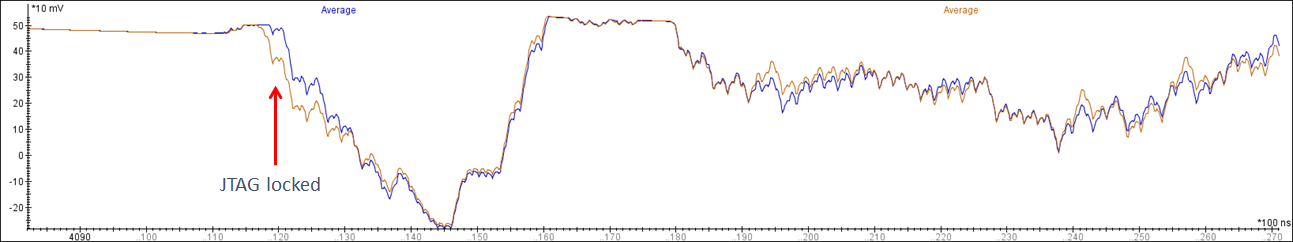
\includegraphics[width=\textwidth]{tms570-DPA-jtag}
  \caption{Difference between locked chip (brown) and unlocked chip (blue) for \TI}
  \label{fig:jtag-ti}
\end{figure*}

\texttildelow259,000 glitches were injected in total for a broad range of different glitch parameters. After tuning the glitch parameters, 35,200 glitches with the optimal parameters were injected. 1.3\% of the attempts succeeded to keep the JTAG unprotected without triggering any lockstep or memory faults. An additional 1.2\% of the glitches succeeded to keep the JTAG unprotected but were detected by the safety mechanisms. Finally, 3.2\% of the attempts had no apparent effects other than triggering the fault detector mechanisms.
This means that the \TI target can be unprotected in less than one minute and half approximately, after performing the preparatory profiling and tuning steps. 

\subsection{\ST}
\ST has several configuration parameters that determine if its debugging interface is locked:
\begin{enumerate}
    \item Life cycle state \label{enum:lifecycle} -- indicates whether the product is still in production or deployed in the field. 
    \item Censorship state \label{enum:censor} -- blocks access to the debugging interface and flash memory. 
    \item Four debug lock bits \label{enum:dbl} -- control access for the different JTAG clients.
\end{enumerate}
The configuration of these parameters is stored in the OTP memory. The default value for those parameters that are not configured is ``locked'' except for the life cycle, which is unlocked by default and has to be configured by the implementor before releasing its final product. Only when all three of these configuration parameters are set to their locked state is the interface properly protected. 

Immediately after the reset and before executing the ROM code, the configuration is pre-loaded by a state machine that reads it from OTP and loads it into the internal configuration registers. A second state machine verifies the written values. An attacker attempting to unprotect the JTAG has to interrupt the pre-load of the life cycle state or, if configured in the final product, the censorship or the debug lock bits. 

The censorship and the debug lock bits are configured as entries or records in a register configuration table stored in OTP. Each record contains a register address and its value. The pre-load state machine iterates through the table and configures the registers. By comparing the power consumption of the boot process with different configuration tables, two points can be identified where the target activity is proportional to the number of records in the table. These points likely correspond to the pre-load and verification operations. Figure \ref{fig:jtag-st} and Figure \ref{fig:jtag-st-2} show the differences for the pre-load and the verification respectively when the table has 2, 102 and 120 records.

\begin{figure*}[!t]
  \centering
  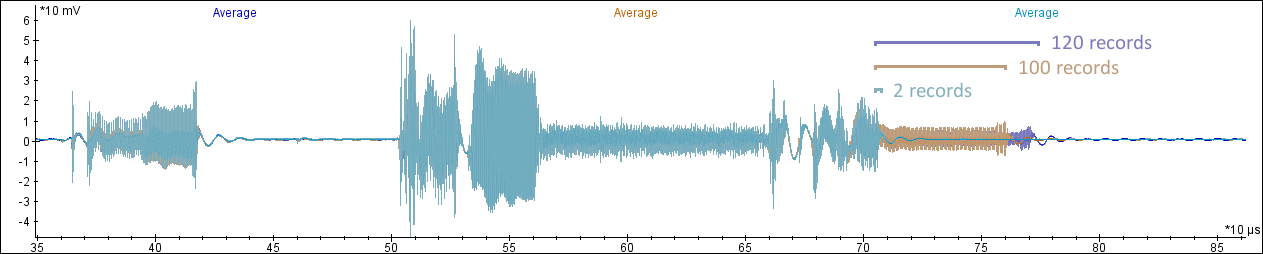
\includegraphics[width=\textwidth]{spc570-DPA-records}
  \caption{Difference between 2 (cyan), 102 (brown) and 120 records (blue) programmed for \ST, point one: load values}
  \label{fig:jtag-st}
\end{figure*}

\begin{figure*}[!t]
  \centering
  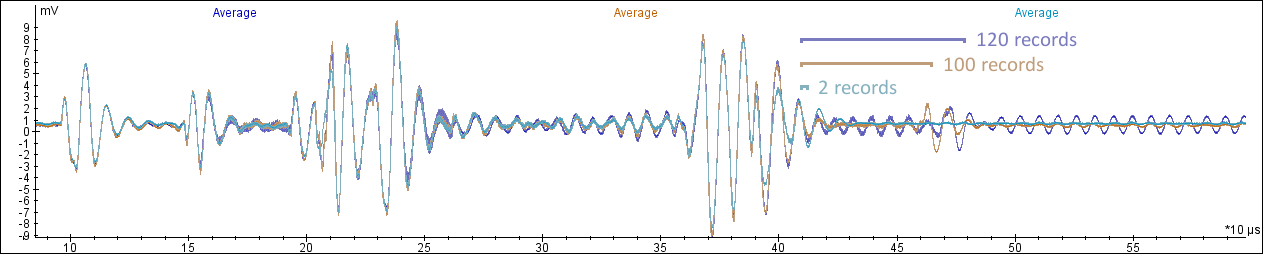
\includegraphics[width=\textwidth]{spc570-DPA-records-2}
  \caption{Difference between 2 (cyan), 102 (brown) and 120 records (blue) programmed for \ST, point two: verify values}
  \label{fig:jtag-st-2}
\end{figure*}

We prepared a target with the censorship and the debug lock bits configured and we ran a FI campaign to glitch the pre-load state machine when iterating the configuration table. As characterization attempts with voltage glitching were unsuccessful, only EM glitching is used for this experiment. After scanning the entire chip surface by injecting \texttildelow240,000 glitches, 0.34\% of the glitches were successful in corrupting debug lock bits configuration. The censorship state was not affected by any glitch. Only a very small part of these glitches, \textless0.001\%, was reported by the module responsible for transferring the records as configuration errors. No more FI campaigns trying to optimize the glitch parameters were ran. The success rate would be higher if optimal parameters where used, especially the position in the chip surface. It is not clear to us why the censorship state was not affected by the glitches and why the verification state machine did not detect more errors.

The life cycle state is not configured using the register configuration table but by writing the value in an OTP register which is directly read by the pre-load state machine. Being able to successfully influence the life cycle state that is configured during boot offers a much more powerful attack than by affecting the censorship or the debug lock bits, as it is not hindered by the circumstantial configuration requirements needed to attack these other parameters.

By comparing the power consumption of the same sample with different life cycle states, differences can be observed in many points during the boot. All these points are potential candidates for glitching to prevent the configuration of the life cycle. We choose to run a FI campaign around the candidate that is closer in time to the spot where we identified that the configuration table was being read. After injecting \texttildelow500,000 glitches, we did not succeed in affecting the life cycle configuration. Further FI campaigns with the other candidates are required to fully discard the possibility of attacking the pre-load of the life cycle.

\subsection{\NXP}
For comparison purposes, the JTAG port of the \NXP chip is also tested. The state of the debug interface is defined by a 32-bit word stored in internal flash, which is read and used by the boot ROM to lock the JTAG port. Because the JTAG configuration word is stored in flash and not in OTP, it can be rewritten multiple times to run a correlation power analysis (CPA). By randomly changing the JTAG configuration word and correlating its Hamming weight with the power consumption, the moment where the ROM reads the configuration word can be find. 

Several voltage FI campaigns are ran to alter the JTAG configuration value read from flash. \texttildelow89,000 glitches are injected in total. In the last campaign, after finding the optimal glitch parameters, 80\% of the \texttildelow10,000 attempts succeeded in unprotecting the JTAG interface, which means that the attack take less than 5 seconds to succeed.


\subsection{JTAG experiments conclusion}
The experiments succeeded in unlocking the JTAG interfaces on the \TI and the \NXP targets, and in the \ST target only when the debug lock bits are configured. Further investigation is needed in order to determine whether the \ST chip can be attacked in other scenarios.
It is not possible to directly compare results on Table \ref{tab:jtag-experiments} because the three chips are implemented with different technologies which could have different sensitivity to FI attacks. Moreover, the experiment on the \ST chip did not attempt to find the optimal glitching parameters to maximize the success rate. In any case, the big gap between success rates between the ASIL and non-ASIL chips indicates that some of the ASIL-D safety mechanisms could slightly mitigate the FI attacks, but cannot fully prevent them.

\begin{table}[!t]
\caption{An overview of the success rates of the different JTAG experiments} 
\label{tab:jtag-experiments}
\centering
\begin{tabular}{p{.06\textwidth} p{.06\textwidth} p{.06\textwidth} p{.06\textwidth}}
\toprule
          
        password \TI
        & lock bits \ST
        & life cycle \ST
        & config \NXP
        \\
    \cmidrule(lr){1-4}          
        1.3\%
        & 0.34\%
        & 0\%
        & 80\%
        \\
\bottomrule
\end{tabular}
\end{table}


\section{Security consequences}
The experiments described in Section \ref{sec:char} and Section \ref{sec:jtag} prove that FI attacks can bypass the detection mechanisms outlined above in state of the art ASIL-D certified MCUs. Although the safety mechanisms detect some faults, they cannot adequately prevent a FI attack.

The fact that it is possible to bypass instructions or execute an unintended branch means that the integrity of the code execution cannot be assured. Any security feature enabled and any check executed in the software can be manipulated by the attacker as an important step toward gaining access to assets. Various assets can be targeted, depending on the attacker profile and the attack scenario. The most common assets include firmware extraction, firmware manipulation, runtime control and access to debug interfaces.

The firmware contained in MCUs is usually the most valuable asset to Tier1 manufacturers and OEMs. The firmware implements those functionalities that add value to the product and differentiate the brand from its competitors. Taking for example a brake controller assistant or an autonomous driving system, there are thousands of hours invested in research and development of the perfect algorithms for stopping the car safely or driving it autonomously through the city. A competitor extracting the software of an ECU would have access to those proprietary technologies and could copy them, or use them to improve their own technology and gain an unfair competitive edge. Extracting the firmware can also be an intermediate step for achieving a bigger objective from a security point of view. An attacker could reverse engineer the extracted software to understand its operation and find a vulnerability. This has been done several times in the past when researchers \cite{garcia_lock_2016,kasper_breaking_2009,verdult_dismantling_2015} reversed the firmware of the remote key entry systems and immobilizers. Vulnerabilities in the cryptographic algorithms were found, which allowed cloning the keys to open and start the car. Similarly, researchers \cite{miller_remote_2015} reversed the extracted software to find remotely exploitable vulnerabilities which gave control of the car without even needing physical access to it.

Modifying the firmware is another common objective of attackers. Typically this attacker profile includes car tuners who seek to modify the performance of their vehicles by altering the software. These persons normally are not aware of the risk that those 
modifications could pose to theirs and others lives. A less common profile could be subjects that are purposely looking to inflict damage in the vehicle or to its occupants by the means of sabotage. In both cases, the possibility of altering the MCU firmware without any tamper evidence is appealing and it should be prevented by the manufacturers. Extracting and modifying the firmware can be done, for example, after bypassing the authentication scheme of the Unified Diagnostic Services (UDS) protocol, if present in the targeted ECU. The authentication experiment described in Section \ref{sec:char} resembles an attack on the UDS authentication.

Runtime control and access to debug interfaces are usually intermediate steps for gaining any of the other assets mentioned. For example, the attack executed in Section \ref{sec:jtag} for gaining JTAG access could be used to extract and modify the firmware in the MCU. An additional benefit of gaining runtime control or debug access is the possibility of experimenting and debugging a live target, which could help to reverse and understand the entire system. Runtime control can be gained using FI through the means of accessing the debug interface, bypassing the Secure Boot or using more advanced techniques like manipulating the CPU's program counter \cite{timmers_controlling_2016}.

Finally, the goal of an FI attack could be simply to disable a security feature. For example, this could be the case for the immobilizer that verifies the response of the key in order to allow starting the engine. By using FI, the attacker could bypass the verification check and start the car without the legitimate key.


\section{Recommendations}
As described before, safety mechanisms implemented in ASIL-D chips can reduce the success rate of FI attacks but not fully prevent them. In the absence of other hardware countermeasures against fault injection, software mitigations like execution flow control, redundancy or random delays should be implemented. The reader can refer to the extensive documentation (e.g. 
\cite{verbauwhede_fault_2011}
) detailing these countermeasures.

It is not only responsibility of the embedded system developers (e.g. Tier1 manufacturers) to implement these countermeasures in their software. As explained in Section \ref{sec:jtag}, ROM code can also be the target of FI attacks and therefore chip manufacturers must also implement countermeasures when developing ROM code. 

When using a MCU with a vulnerable ROM, embedded system developers can mitigate the risk by using the ROM patching mechanism, if such a mechanism is present. For example, ARM Cortex MCUs usually implement the Flash Patch and Breakpoint Unit (FPB) which can be used to patch ROM code. Depending on the MCU manufacturer, the FPB can be enabled at reset time and patch the boot routine, or can only be enabled after booting and patch only the ROM drivers used in the application. In the experiment performed on \TI described in Section \ref{sec:jtag}, 1.2\% of the glitching attempts succeeded to unprotect the debug interface protection mechanism, but lockstep or memory errors were detected. The application developers should check for these errors or any other unexpected state (e.g. unexpected values in a JTAG configuration register) immediately after booting and reset the chip if any inconsistency is found. 
In the specific case of the \ST target, adding redundant records to configure the censorship and the debug lock bits could mitigate an FI attack on them.


\section{Future work}
This work leaves several open questions that are interesting for future work:

\begin{itemize}
  \item Perform similar investigations on additional targets that implement these safety mechanisms to further identify their effectiveness as countermeasures.
    \item Apply fault injection attacks on real world systems using ASIL-D MCUs (i.e. ECUs) to confirm that these attacks pose a real threat. It is especially interesting to test implementations of the UDS authentication scheme. 
    \item Test targets that allow disabling and tuning the safety mechanisms individually and characterize the effectiveness of each mechanism. For example, all targets tested in this work use a two-clock cycles delay between the two lockstep cores. Different delays might be more or less effective.
    \item Do additional characterization experiments with the presence of software countermeasures. This should give an insight in what type of setup would be better in combating fault injection attacks.
\end{itemize}

\section{Conclusion}
We assessed the resistance of two ASIL-D MCUs against fault injection attacks using both voltage and EM glitching techniques. Both targets appeared highly sensitive to at least one of these techniques in our characterization experiments, showing that basic conditional branch type code structures can successfully be attacked in ASIL-D targets. Furthermore, we succeeded in identifying and attacking the JTAG protection by using power analysis and voltage glitching in one ASIL-D and one QM target and extracted secret information from its firmware. Limited success was obtained attacking the JTAG protection of the second ASIL-D target. Each experiment required approximately one week of preparation, but once the attacker finds the optimal glitching parameters, the attack can be repeated in less than an hour, including the time needed to modify the application PCB.

We observed that, compared to standard non-ASIL MCUs, the safety mechanisms implemented in ASIL-D chips can help to mitigate fault injection attacks, but not fully prevent them, nor can they reduce the risk that these attacks pose to an acceptable level. We advise MCU manufacturers and embedded system developers to implement both hardware and software countermeasures against fault injection.

\newpage
% trigger a \newpage just before the given reference
% number - used to balance the columns on the last page
% adjust value as needed - may need to be readjusted if
% the document is modified later
%\IEEEtriggeratref{8}
% The "triggered" command can be changed if desired:
%\IEEEtriggercmd{\enlargethispage{-5in}}

% references section

% can use a bibliography generated by BibTeX as a .bbl file
% BibTeX documentation can be easily obtained at:
% http://www.ctan.org/tex-archive/biblio/bibtex/contrib/doc/
% The IEEEtran BibTeX style support page is at:
% http://www.michaelshell.org/tex/ieeetran/bibtex/
\bibliographystyle{IEEEtran}
% argument is your BibTeX string definitions and bibliography database(s)
\bibliography{IEEEabrv,refs}

% that's all folks
\end{document}


